\documentclass[aspectratio=169]{beamer}
%% For 4:3 aspect ratio:
%% \documentclass{beamer}
\usepackage{../git-course}

\title[git-course]{Git details}
\author{Chris Grandin \& Andy Edwards}
\date{\today}

\begin{document}

\frame[plain]{
\titlepage
}

\section{Introduction}
\frame{\frametitle{Commits and history}
  Git does not keep versions of software, it keeps \emph{commits}. The commits
  are kept track of using a hash code, using \emph{Secure Hash Algorithm 1}
  (SHA-1) which generates a hash key 40 digits long in hexadecimal. These are
  what you see on \gh\ and in various places when you use \gs.\\
  \bigskip
  Several of these commits have pointers to them which have special names:
  \bi
    \item the \textbf{HEAD} which points to the commit you are currently on
      in the \gs.
    \item the \textbf{master} which is just another branch and is the default
      one when you set up a repository on \gh.
    \item the branch names that you have in your repository.
  \ei
  Once you've cloned a \gh\ repository, the \emph{master} points at the initial
  commit, and the \emph{HEAD} points at the master.
}

%% Figures from : https://marklodato.github.io/visual-git-guide/index-en.html?no-svg

\frame{\frametitle{Git layout}
  \begin{columns}
    \begin{column}{0.4\linewidth}
      \bi
        \item \textcolor{green}{Green} items are commits.
        \item \textcolor{orange}{Orange} items are branches.
        \item The \textcolor{blue}{Stage} holds references to files you have
          added using \lstinline{git add FILE-NAME} for the next commit.
        \item The current branch is always pointed to by \textbf{HEAD}.
        \item \textbf{ed489} is the most recent commit, and it is pointed to
          by \textbf{master} and \textbf{HEAD}.
        \item \textbf{maint} is another branch, and is an ancestor of
          \textbf{master}.
      \ei
    \end{column}
    \begin{column}{0.6\linewidth}
      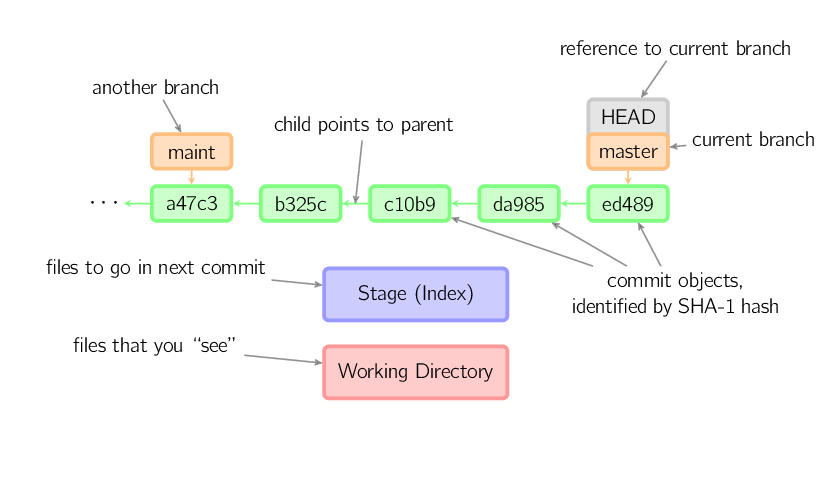
\includegraphics[
        width=\textwidth,
        height=0.8\textheight,
        keepaspectratio]
                      {figures/head-master}
    \end{column}
  \end{columns}
}

\frame{\frametitle{Commit on master}
  \begin{columns}
    \begin{column}{0.4\linewidth}
      \bi
        \item When you do a \lstinline{git commit} while in the \textbf{master}
          branch, \textbf{master} and \textbf{HEAD} are moved up one to point
          at the new commit. Everything else remains the same.
        \item Any files you want included in the new commit must be have been
          added previously with the \lstinline{git add FILENAME} command so
          that they are in the \textcolor{blue}{Stage} area for the commit.
      \ei
    \end{column}
    \begin{column}{0.6\linewidth}
      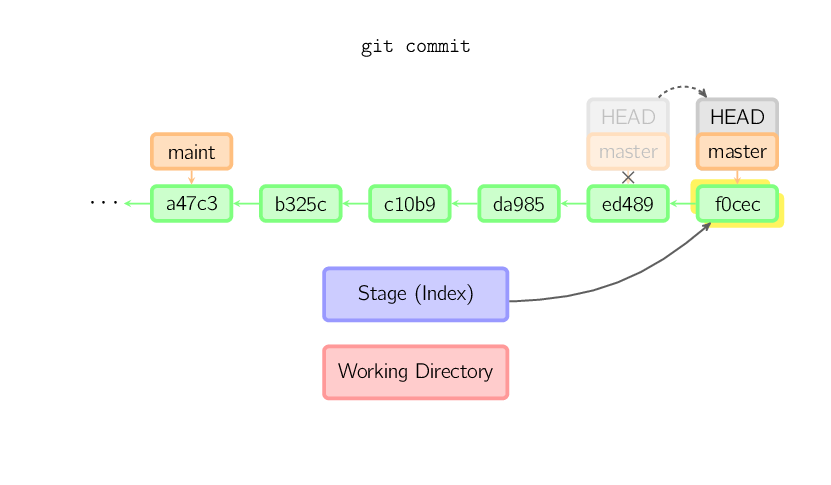
\includegraphics[
        width=\textwidth,
        height=0.8\textheight,
        keepaspectratio]
                      {figures/commit-master}
    \end{column}
  \end{columns}
}

\frame{\frametitle{Commit on another branch}
  \begin{columns}
    \begin{column}{0.4\linewidth}
      \bi
        \item If you have changed to another branch using
          \lstinline{git co maint} and then commit changes, \textbf{maint}
          and \textbf{HEAD} will be moved up to the new commit, \textbf{1800b}.
        \item \textbf{maint} is no longer an ancestor of \textbf{master}.
        \item Any files added will be a part of the \textbf{maint} branch
          and will not appear in the \textbf{master} branch.
      \ei
    \end{column}
    \begin{column}{0.6\linewidth}
      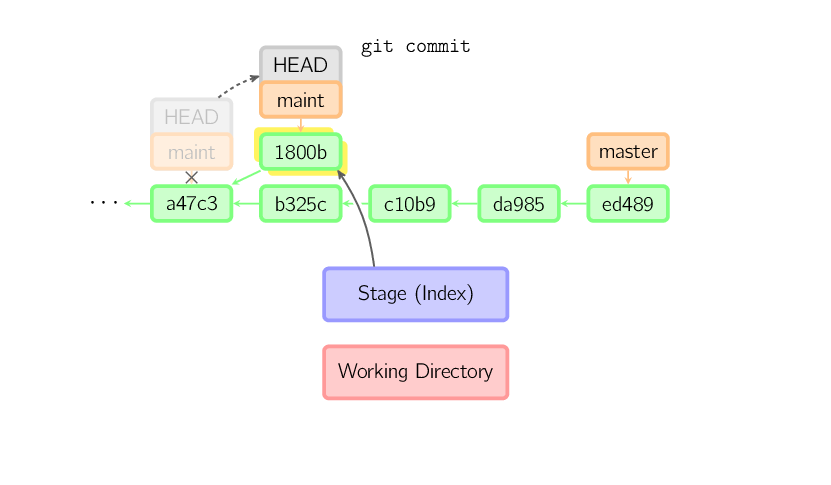
\includegraphics[
        width=\textwidth,
        height=0.8\textheight,
        keepaspectratio]
                      {figures/commit-maint}
    \end{column}
  \end{columns}
}

\frame{\frametitle{Commit amendment}
  \begin{columns}
    \begin{column}{0.4\linewidth}
      \bi
        \item If a mistake is made in the last commit, you can use
          \lstinline{git commit --amend}.
        \item it creates a new commit (\textbf{4ca87}) and discards the old
          one if nothing else is pointing to it (\textbf{ed489}).
        \item \textbf{master} and \textbf{HEAD} will be moved up to the
          new commit.
      \ei
    \end{column}
    \begin{column}{0.6\linewidth}
      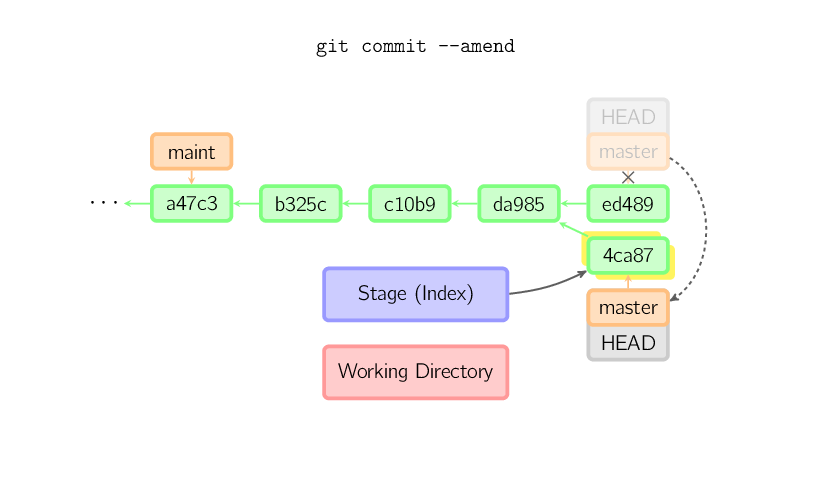
\includegraphics[
        width=\textwidth,
        height=0.8\textheight,
        keepaspectratio]
                      {figures/commit-amend}
    \end{column}
  \end{columns}
}

\frame{\frametitle{Checking out at any commit}
  \begin{columns}
    \begin{column}{0.4\linewidth}
      \bi
        \item You can go to any commit and see how things looked at that
          point in time. \lstinline{git checkout b325c} or
          \lstinline{git checkout master~3} will put your \textbf{HEAD} in this
          position.
        \item Your working directory will change structure to be exactly
          what is was at that commit.
        \item This is the same as changing to another branch, but there
          is no branch reference, leaving you in a \textbf{Detached Head}
          state.
      \ei
    \end{column}
    \begin{column}{0.6\linewidth}
      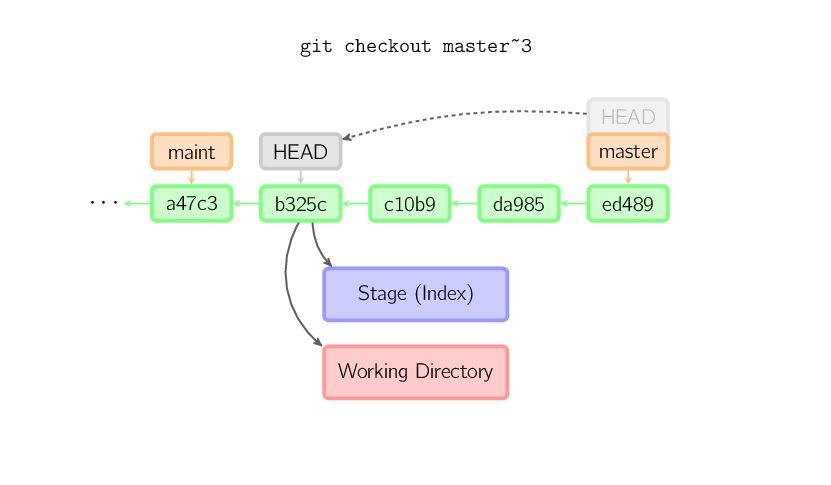
\includegraphics[
        width=\textwidth,
        height=0.8\textheight,
        keepaspectratio]
                      {figures/detached-head}
    \end{column}
  \end{columns}
}

\frame{\frametitle{Committing with a detached \textbf{HEAD}}
  \begin{columns}
    \begin{column}{0.4\linewidth}
      \bi
        \item Commits work as usual, but there is no named branch so if you
          use the \lstinline{git checkout} command after committing in a
          detached HEAD state, you will
          \textbf{lose all the work in those commits}.
        \item To avoid losing these commits, save your commits before changing
          back to \emph{master} or another branch by creating a new branch
          where you currently are.
      \ei
    \end{column}
    \begin{column}{0.6\linewidth}
      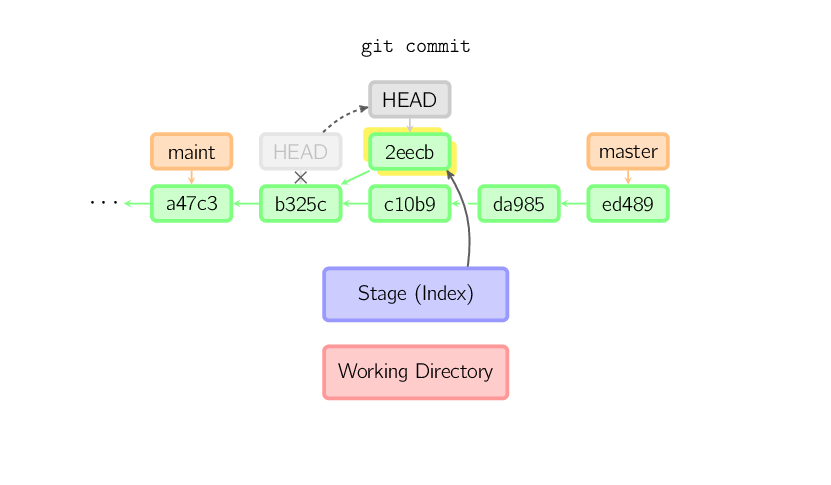
\includegraphics[
        width=\textwidth,
        height=0.8\textheight,
        keepaspectratio]
                      {figures/commit-detached}
    \end{column}
  \end{columns}
}

\frame{\frametitle{Creating a branch while in a detached \textbf{HEAD} state}
  \begin{columns}
    \begin{column}{0.4\linewidth}
      \bi
        \item Creating a branch while in a detached HEAD state will change you
          to the new branch and take you out of the detached HEAD state:\\
          \lstinline{git checkout -b BRANCH-NAME}\\
          or use the alias:\\
          \lstinline{git cb BRANCH-NAME}
      \ei
    \end{column}
    \begin{column}{0.6\linewidth}
      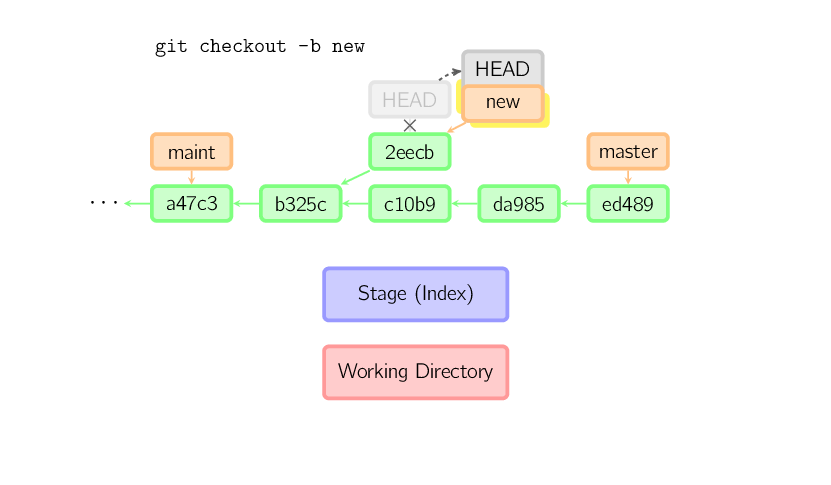
\includegraphics[
        width=\textwidth,
        height=0.8\textheight,
        keepaspectratio]
                      {figures/checkout-b-detached}
    \end{column}
  \end{columns}
}

\frame{\frametitle{Advanced stashing}
  You can stash more than one set of changes if you wish. To see your list
  of available stashes:\\
  \lstinline{git stash list}\\
  The list will look something like this:\\
  \lstinline{stash@\{0\}: WIP on master: 46ae7a8 Merge conflict resolved.}\\
  \lstinline{stash@\{1\}: WIP on master: fe35a9b Minor change to Readme.}\\
  \lstinline{...}\\
  where each commit the stash was based on is listed. You can apply any
  of these by using the syntax:\\
  \lstinline{git stash apply stash@\{N\}}\\
  where N is one of the numbers shown. If you don't specify a stash, the
  most recent one is used.
}

\end{document}
